\chapter{Theoretical Background}
\label{chapter:background}
\section{Molecular Orbital Theory}
\label{sec:MO_theory}
In order to understand the bonding in organometallic systems, we first have to understand the theoretical background of electron structure in molecules. This strucutre of this section is based on these books \cite{atkins2011molecular, albright2013orbital}. We start of with the time-independent Schr\"odinger equation, which describes the energy of a system as:
\begin{equation}
    \hat{H}\Psi(r) = E\Psi(r),
    \label{eq:Schroedinger_equation}
\end{equation}
where $\hat{H}$ is the Hamilton operator, $\Psi$ is the wavefunction of the system at the position $r$ in space, and $E$ is the total energy of the system. The Hamiltonian is given as the sum of the operator for kinetic energy $\hat{T}_{kin}$ and potential energy $\hat{V}$, which can be rewritten as:
\begin{equation}
    \hat{H} = \hat{T}_{kin} + \hat{V}.
    \label{eq:Hamilton_operator}
\end{equation}
Solving the Schr\"odering equation in spherical coordinates yields the following wavefunction:
\begin{equation}
    \Psi_{n, l, m}(r, \theta, \phi) = R_{n, l}(r)Y_{l}^{m}(\theta, \phi),
    \label{eq:soltion_hydrogen}
\end{equation}
which is product of $R_{n, l}(r)$, related to the Laguerre functions, depending only on the distance $r$, and $Y_{l}^{m}(\theta, \phi)$, which is a spherical harmonic, containing all angular information \cite{atkins2011molecular}. Here, $n$ is the principle quantum number, $l$ is the angular momentum quantum number, and $m$ is the magnetic quantum number. The Schr\"odering equation can only be exactly solved for one-electron systems (e.g., H, Li$^{2+}$). In the specific case of one-electron wavefunctions they are called atomic orbitals (AO). For historical reasons, orbitals with $l$ = 0, 1, 2, and 3 are termed s-, p-, d- and f-orbitals, respectively. An electron by a given one-electron wavefunction $\Psi_{n, l, m}$ can be understood as occupying that orbital and referred to as and s-, p-, d- and f-electron. \\
As for systems with more than one electron the Schr\"odinger equation cannot be solved, an approximation has to be introduced to the describe the electronic structure for many-electron systems, especially molecules. Molecular orbitals (MOs) can be approximated as a linear combination of atomic orbitals (LCAO ansatz):
\begin{equation}
    \psi_{i} = c_{1i}\phi_{1} + c_{2i}\phi_{2} + \cdots + c_{mi}\phi_{m} = \sum_{a}c_{ai}\phi_{a},  
    \label{eq:LCAO_ansatz}
\end{equation}
where the index $i$ ranges from 1 to $m$ which is the total number of basis functions. $\phi$ are the atomic basis functions and $c_{ai}$ are the molecular orbital coefficients. These MOs are one-electron wavefunctions and are orthonormal (i.e. normalized and orthogonal)
\begin{equation}
    \braket{\psi_{i}|\psi_{j}} = \delta_{ij},
    \label{eq:orthonormality}
\end{equation}
where $\delta_{ij} = 1$ for $i = j$ and $\delta_{ij} = 0$ for $i \neq j$. The molecular orbital coefficients $c_{ai}$ act as scaling factor of the $a$th atomic orbital and specify the nature and energy of the orbital $\psi_{i}$. They are determined by solving the eigenvalue equation of the effective one-electron Hamiltonian $\hat{H}^{\mathrm{eff}}$ associated to the molecule:
\begin{equation}
    \hat{H}^{\mathrm{eff}}\psi_{i} = \epsilon_{i}\psi_{i}.
    \label{eq:one_electron_Hamiltonian}
\end{equation}
Here, $\epsilon_{i}$ is the molecular orbital energy of the an electron located in $\psi_{i}$, which can be calculated as the expectation value of $\hat{H}^{\mathrm{eff}}$.
\begin{equation}
    \epsilon_{i} = \bra{\psi_{i}}\hat{H}^{\mathrm{eff}}\ket{\psi_{i}}
    \label{eq:MO_energy}
\end{equation}
Before we continue with this formalism, we introduce the overlap integral $S_{\mu \nu}$ between two atomic orbitals $\phi_{\mu}$ and $\phi_{\nu}$:
\begin{equation}
    S_{\mu \nu} = \braket{\phi_{\mu}|\phi_{\nu}},
    \label{eq:overlap_integral}
\end{equation}
which describes the spatial overlap of two wavefunctions (here in Figure \ref{fig:overlap_integral} the overlap of two 1s orbitals).
\begin{figure}[H]
    \centering
    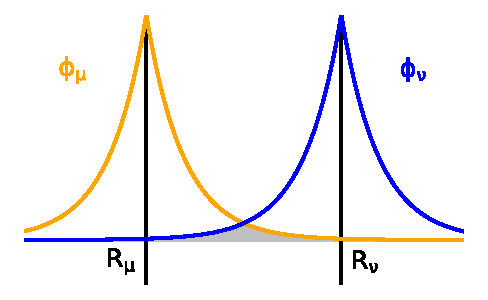
\includegraphics[width=0.5\linewidth]{Figures/Overlap_integral.pdf}
    \caption{Spatial overlap of wavefunctions of two 1s orbitals having the same phase. The atomic orbitals have their origin at R$_{\mu}$ and R$_{\nu}$. The gray shaded area indicates the overlapping area between the two wavefunctions.}
    \label{fig:overlap_integral}
\end{figure}
\noindent
The interaction between two orbitals with each other is quantified in the magnitude of the overlap integral, serving as a powerful tool in the detailed analysis of molecular orbitals. Especially the symmetry of the atomic orbitals is of great importance in dictating whether the overlap integral is zero or not. Figure \ref{fig:symmetry_MOs} shows an overview of various types of overlap integrals. $\sigma$-symmetric orbital overlap is characterized by the absence of nodes along the internuclear axis, whereas $\pi$-symmetric overlap contains a single node, and $\delta$-symmetric contains two nodes along the axis. Nodes along the internuclear axis decrease the overlap between orbitals, which results in a decrease of the overlap integral according to $\sigma > \pi > \delta$. This general rule of thumb is only valid for valence orbitals of atoms from the same row of the periodic table \cite{albright2013orbital} and depends strongly on the spatial extend of the respective atomic orbitals.
\begin{figure}[H]
    \centering
    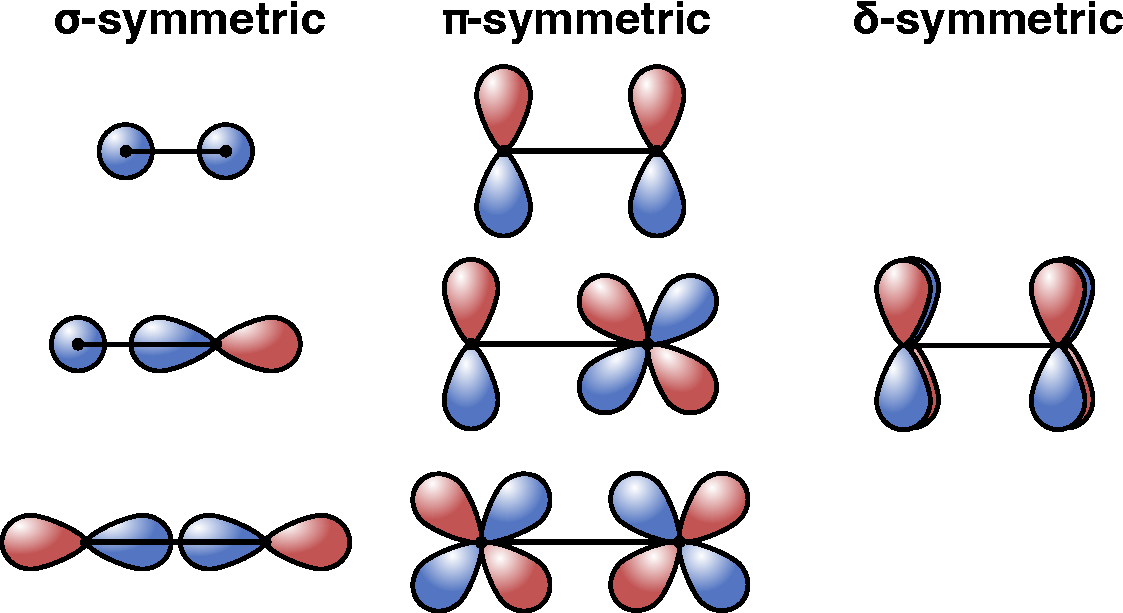
\includegraphics[width=0.8\linewidth]{Figures/Symmetry_orbitals.pdf}
    \caption{Examples of different types of overlap between atomic orbitals. }
    \label{fig:symmetry_MOs}
\end{figure}
\noindent
Another aspect influencing the overlap, is the principle quantum number $n$ of the atomic orbitals. As $n$ increases, the atomic orbitals become more diffuse which normally decreases the overlap. Moreover, the orbital overlap is highly sensitive to the internuclear distance between atoms as well as to the electronegativity, where less electronegative atoms exhibit more diffuse orbitals. An important exception to the generalization discussed above occurs in transition metal complexes. The 3d orbitals are relatively contracted due to their poor radial extension and ineffective shielding by inner electrons. At typical metal-ligand distances, this contraction reduces their spatial overlap with ligand orbitals. In contrast, 4d and 5d valence orbitals are radially more extend as a result of stronger shielding of the positive charge of their nucleus, and therefore exhibit greater overlap with ligand orbitals. Last, the overlap is very sensitive to the geometry of the molecule.
\\Coming back to equation \ref{eq:LCAO_ansatz}, in order to get the optimum value for the orbital coefficients $c$ the variation principle is applied, which leads to the problem of solving the secular equations (an exact derivation can be found here \cite{albright2013orbital}):
\begin{equation}
    \sum_{a} c_{ai}\left(\hat{H}_{\mu\nu}-\epsilon_{i}S_{\mu\nu}\right), 
    \label{eq:secular_equations}
\end{equation}
where $\hat{H}_{\mu\nu}$ is a matrix element of the Hamiltonian and the index $i$ indicates the molecular orbital level. The Hamiltonian is given as:
\begin{equation}
    \hat{H}_{\mu\nu} = \braket{\phi_{\mu}|\hat{H}^{\mathrm{eff}}|\phi_{\nu}}.
    \label{eq:hamiltonina_matrix_element}
\end{equation}
The secular equations \ref{eq:secular_equations} can be express in matrix form as the following:
\begin{equation}
    \textbf{H} \vec{c} = \epsilon \textbf{S}\vec{c}.
    \label{eq:matrix_eigenvalue_problem}
\end{equation}
This is a matrix eigenvalue problem, which represents the formulation of quantum mechanics by Heisenberg. The advantage of this approach is the transformation of differential equations into an algebraic eigenvalue problem, which can be solved efficiently by computer algorithms. Here, \textbf{H} is the Hamiltonian matrix of elements $\hat{H}_{\mu\nu}$, $\vec{c}$ is the coefficient vector containing all unknown orbital coefficients $c_{i}$, $\epsilon$ is the diagonal matrix of energies $\epsilon_{i}$, \textbf{S} is the overlap matrix containing $S_{\mu\nu}$. \\
Solving the eigenvalue equation gives the orbital coefficients and makes the construction of MOs according to LCAO ansatz (see equation \ref{eq:LCAO_ansatz}). For the example of a degenerate interaction, so two atomic orbitals with the same energy, we get the two following MOs:
\begin{align}
    \psi_{1} = \frac{1}{\sqrt{2+2S_{12}}}\left(\phi_{1}+\phi_{2}\right) \\
    \psi_{2} = \frac{1}{\sqrt{2-2S_{12}}}\left(\phi_{1}-\phi_{2}\right)
    \label{eq:MOs_degenerate_interaction}
\end{align}
Here, $\psi_{1}$ is the bonding MO, formed by the in-phase combination of the atomic orbitals $\phi_{1}$ and $\phi_{2}$, whereas $\psi_{2}$ is the anti-bonding MO, formed by the out-of-phase combination. They are depicted in a molecular orbital diagram in Figure \ref{fig:MO_diagrams}a together with the case of nondegenerate interaction (Figure \ref{fig:MO_diagrams}b). The derivation of the analytic expression of those MOs will not be covered here, but can be found in the literature \cite{albright2013orbital}.
\begin{figure}[H]
    \centering
    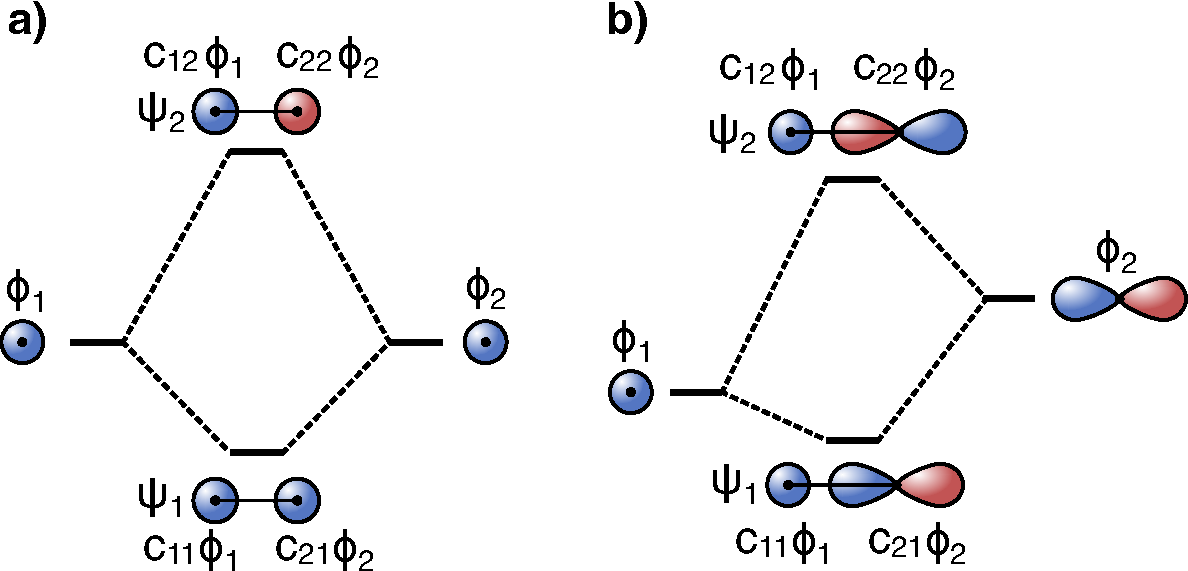
\includegraphics[width=0.95\linewidth]{Figures/MO_diagram_degenreate_and_non_degenerate.pdf}
    \caption{Molecular orbital diagram of a) the degenerate interaction between two atomic s orbitals and b) the non-degenerate interaction between a atomic s and p orbital. The atomic orbitals are denoted as $\phi_{1}$ and $\phi_{2}$ and their in-phase and out-of-phase combination as $\psi_{1}$  and $\psi_{2}$, respectively. The first index of the orbital coefficients indicates the atom and the second the corresponding MO.}
    \label{fig:MO_diagrams}
\end{figure}
\noindent
Until here, we have only considered the two-orbital problem, which is extremely powerful as many bonding situations in chemistry can be reduced into this from. General trends of orbital interactions in this picture can be summarized as the following:
\begin{enumerate}
    \item The upper MO (out-of-phase combination, antibonding) is destabilized more than the lower MO (in-phase combination, bonding).
    \item The magnitude of the interaction energy (MO splitting) increases with increasing overlap of the atomic orbitals.
    \item In nondegenerate orbital interaction, the magnitude of the interaction energy is inversely proportional to the energy difference of the interacting orbitals. The character of a molecular orbital most closely reflects that of the atomic orbital nearest to it in energy.
\end{enumerate}
To get molecular orbitals of polyatomic species, the same LCAO ansatz (see eqauation \ref{eq:LCAO_ansatz} can be utilized with the sum ranging over all atomic molecules of the atoms in the molecule. Similar to the two-orbital example, only atomic molecules with appropriate symmetry can contribute due to their net overlap. \\
With this key concept introduced, we are now able to utilize molecular orbitals to explain the bonding in metal organic complexes, which will be the topic of the next section.

\section{Organometallic Bonding}
\label{sec:Organometallic_Bonding}
Organometallic complexes comprise a vast array of metals, oxidation states, and ligands and thus enable a wide variety of structures and unique bonding motives, which provide the foundation for the reactivity and stability. Thus, it is important to introduce the fundamental principles to understand their unique behavior. We will focus here in particular on organometallic complexes using transition metals. A complete and detailed description of the underlying interactions can be found in the literature \cite{Hartwig_book, albright2013orbital}.
\subsection{Types of Organometallic Bonding}
\label{subsec:types_organometallic_bonding}
In general, a transition metal complex consists of a central transition metal atom which is surrounded by molecules or atoms which are called ligands. An important formalism in organometallic bonding is the determination of the number of electrons of the ligand involved in the bonding to the metal. This interaction are to large extend Lewis acid-base (electron acceptor and donor) interactions, in which the metal often acts as a Lewis acid and the ligand as a Lewis base. This interaction can occur through different modes of orbital overlap between the ligand and metal, with the two most fundamental being $\sigma$-bonding and $\pi$-bonding, which have there name due to the symmetry requirements of the orbitals involved in these interactions (see Figure \ref{fig:symmetry_MOs}). These different bonding motives are schematically shown in Figure \ref{fig:Bonding_in_metal_complexes}.
\begin{figure}[H]
    \centering
    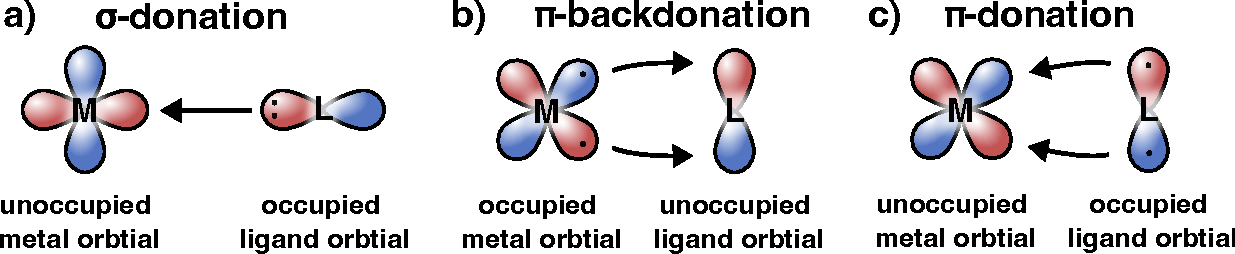
\includegraphics[width=0.95\linewidth]{Figures/Bonding_in_metal_complexes.pdf}
    \caption{Schematic and generalized orbital interactions for a) $\sigma$-donation, b) $\pi$-donation, and c) $\pi$-backdonation in organometallic complexes.}
    \label{fig:Bonding_in_metal_complexes}
\end{figure}
\noindent
In $\sigma$-bonding, the interaction between the ligand and metal arises from the overlap of a filled ligand orbital with metal orbital along the internuclear axis. In most case electron density from a ligand lone pair (e.g. in phosphines or amines) is donates into an empty metal orbital, increasing thereby the electron density at the metal center. Ligands exhibiting such bonding are called $\sigma$-donors. A more special case of $\sigma$-bonding will be discussed in greater detail in section \ref{subsec:sigma_complexes}.\\
In $\pi$-bonded ligands, the involved orbitals of the ligand and metal are oriented perpendicular to the internuclear axis. The interaction between can be divided into $\pi$-donation and $\pi$-back-donation. We focus first on $\pi$-backdonation, in which electron density is transferred from an occupied metal d-orbital into an unoccupied ligand orbital. This interaction is extremely important for the stabilization of complexes with metals in a low formal oxidation states. Most prominent examples for this interaction are carbon monoxide (CO) or nitrosyl cation (NO$^{+}$) which act as strong electron acceptors using their unoccupied $\pi^{*}$-orbitals. This donation of electron density from the metal to the $\pi^{*}$-orbital is know as "backbonding". This destabilizing interaction is more than compensated by the reduced electron density at the metal. In $\pi$-donation, electron density is transferred from an occupied ligand orbital into an empty metal d-orbital, analogous to $\sigma$-donation but involving orbitals oriented perpendicular to the metal-ligand axis. Typical $\pi$-donor ligands are aromatic systems like arenes. In general, these different bonding motives can appear in a single ligand, as long as the symmetry requirements are met for the interactions. However, there relative magnitude is influenced by the electronic structure of the ligand itself. 

\subsection{Sigma-Complexes}
\label{subsec:sigma_complexes}
A special type of metal-ligand interaction occurs in so-called $\sigma$-complexes, in which neutral molecules like dihydrogen, alkanes, silanes and boranes are bound through their H-H, C-H, Si-H or B-H bonds, respectively. Here, we will focus mainly on the case of $\sigma$-alkane complexes as they are the key intermediate in activation of C-H bonds via oxidative addition. The C-H bond binds to the transition metal complex in a combination of two charge transfer interactions (see Figure \ref{} \textcolor{red}{SHOULD I REALLY DO THIS?}), which were first conceptualized on an orbital level by Saillard and Hoffmann \cite{saillard1984carbon}. 
On the one hand, electron density is donated via ligand-to-metal charge transfer (LMCT) from the occupied C-H $\sigma$-orbital to unoccupied metal d-orbitals. On the other hand, electron density is donated in parallel from occupied metal d-orbitals to the unoccupied C-H $\sigma^{*}$-orbital (metal-to-ligand charge transfer, MLCT), acting in the opposite direction. These interactions resemble $\sigma$-donation and $\pi$-backbonding, respectively. The combination of this bidirectional interactions weakens the C-H bond, thereby facilitating C-H activation. Modulation of the metal center's electronic structure plays an important role in enabling the formation of such intermediates and ultimately governs their reactivity in subsequent oxidative addition steps.
\section{Photochemical C-H Activation using Transition Metal Complexes}
\begin{itemize}
    \item examples of C-H activation, small historical back ground
    \item other mechanisms besides C-H activation via sigma complex formation and oxidative addition
    \item reactivity in C-H activation, Hartwig trends, hoffmann sailard explained in detail
\end{itemize}
\textcolor{red}{STILL WRITE THIS STUFF}